\chapter{Eletrônica}
\label{eletronica}

\section{Microcontrolador} % (fold)
\label{sec:msp430}

% É um microcontrolador RISC de 16 bits criado pela Texas Instrumets para aplicações de baixo consumo de energia.
O microcontrolador utilizado neste projeto foi o MSP430G2553. Este microcontrolador possui uma arquitetura RISC com registradores de 16 \textit{bits} e 27 instruções, 512 \textit{Bytes} de RAM e pode operar com um \textit{clock} de até 16MHz. As aplicações foram trabalhadas a partir da plataforma MSP430 \textit{Launchpad}. Esta plataforma foi desenvolvida pela \textit{Texas Instruments} (TI) como um \textit{kit} de avaliação para microcontroladores da linha MSP430G. Este microcontrolador apresenta algumas características importantes para a realização deste trabalho. São elas:
\begin {itemize}
	\item 2 \textit{Timers} (TA0 e TA1) com 16 \textit{bits} e 4 modos de contagem;
	\item 8 canais de entrada para um Conversor A/D de 10\textit{bits} ( ADC10 tipo SAR);
	\item Serviços de interrupção por \textit{Hardware};
	\item \textit{Hardware} de comunicação serial com suporte para UART.
\end {itemize}

\begin{figure}[h]
  \centering
  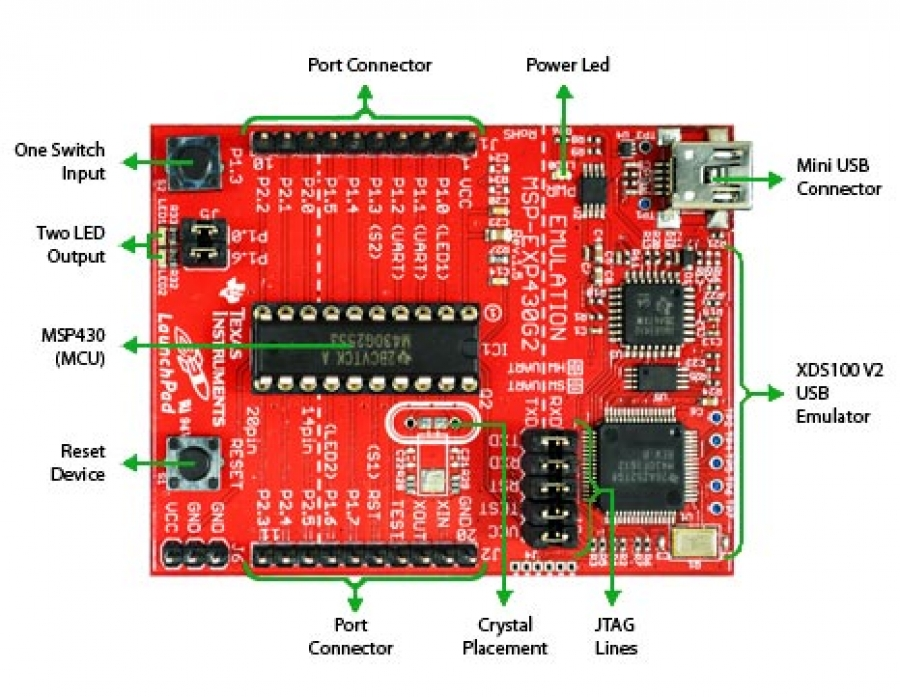
\includegraphics[width=0.6\textwidth]
      {figuras/Launchpad.jpg}
  \caption{Pataforma para desenvolvimento MSP430 \textit{Launchpad}.}
  \label{Launchpad}
\end{figure}
% Colocar aqui sobre o que é o MSP430, sua função no projeto como foi utilizado
Em comparação com outras plataformas, como o Arduino, a MSP430 \textit{Launchpad} apresenta um menor custo. A plataforma Arduino apresenta mais facilidade para a implementação de protótipos através de sua linguagem de programação na Arduino IDE, porém, a plataforma \textit{Launchpad} também possuí uma plataforma similar disponível chamada de \textit{Energia}. Neste projeto, entretanto, optou-se por utilizar a ferramenta msp430-gcc e mspdebug para desenvolver as aplicações de software embarcado e programar o dispositivo respectivamente. Elas foram escolhidas por possibilitar mais liberdade de desenvolvimento no microcontrolador e possibilidade de seguir em nível mais próximo do \textit{hardware}, apesar da maior complexidade na elaboração das aplicações.


%\subsection{MSPGCC} % (fold)
%\label{sub:mspgcc}

%É um porte do \textit{GNU C Compiler} (\textbf{GCC}) e do \textit{GNU Binutils} (\textbf{as}, \textbf{ld}) para o microcontrolador \textit{MSP430}. São providenciadas ferramentas para depuração e \textit{download} de binário (\textbf{GDB, JTAG} e \textbf{BSL}).

% Item sobre a visão sistemica da eletronica embarcada

\subsection{Arduindo}
\label{sec:arduino}

O Arduino é plataforma \textit{open-source} criada de forma a facilitar o uso da integração de \textit{software} e \textit{hardware}. Foi utilizado o microcontrolador Arduino Mega que é baseado no Atmega 1280. Tem-se um total de 54 pinos digitais de entrada e saída no qual 14 deles tem a possibilidade de serem usados como um sinal PWM (\textit{Pulse Width Modulation}), 16 pinos para entrada de sinais analógicos, 4 portas para comunicação UART (\textit{Universal asynchronous receiver/transmitter}), um oscilador de cristal de 16 MHz, uma conexão USB, uma entrada de alimentação e um botão de \textit{reset}.

O ATmega1280 possui 128 KB de memória \textit{flash} para armazenamento de código (dos quais 4KB são usados pelo \textit{bootloader}), 8 KB de SRAM e 4 KB de EEPROM (que poder ser lidos e escritos com a biblioteca EEPROM). Outra característica importanta é a quantidade de portas de entrada e saída disponíveis, o que permitiu uma maior liberdade ao receber os sinais dos sensores; 



\section{Visão Sistêmica da Eletronica Embarcada} % (fold)
\label{sec:visao_sistemica}

No ponto de vista da eletrônica embarcada, enxergam-se dois pontos principais: O PC com o ambiente virtual e os sensores e atuadores instalados na bicicleta. O primeiro destes realizará o processamento do ambiente virtual a partir dos dados obtidos pelos sensores e atualizando a posição do ciclista no ambiente. Em seguida, devolverá como sinal de retorno à bicicleta no controle do freio para transmitir uma sensação de peso ao ciclista. Para tornar isso possível, trabalhou-se com 2 sensores e um atuador, listados a seguir.


\begin {itemize}
	\item Posição do guidão;
	\item Velocidade da roda.
	\item Servo motor.
\end  {itemize}

Neste contexto, o sistema de software embarcado foi projetado baseando-se no diagrama de blocos apresentado na Figura \ref{blocos}. O sensor de posição do guidão se trata de um potenciômetro comum com variação de ângulo de 0 a 270 graus e 0 a 10 k$\Omega$ de variação de resistência proporcional ao ângulo. O sensor de velocidade se trata de um conta giros através de interferência entre um par transmissor-receptor de infravermelho que permitirá verificar o movimento da roda traseira. O atuador constante em um servomotor cuja posição será controlada de forma a controlar o freio da bicicleta, aumentando o atrito com a roda traseira e fornecendo uma sensação de peso ao usuário.

\begin{figure}[h]
  \centering
  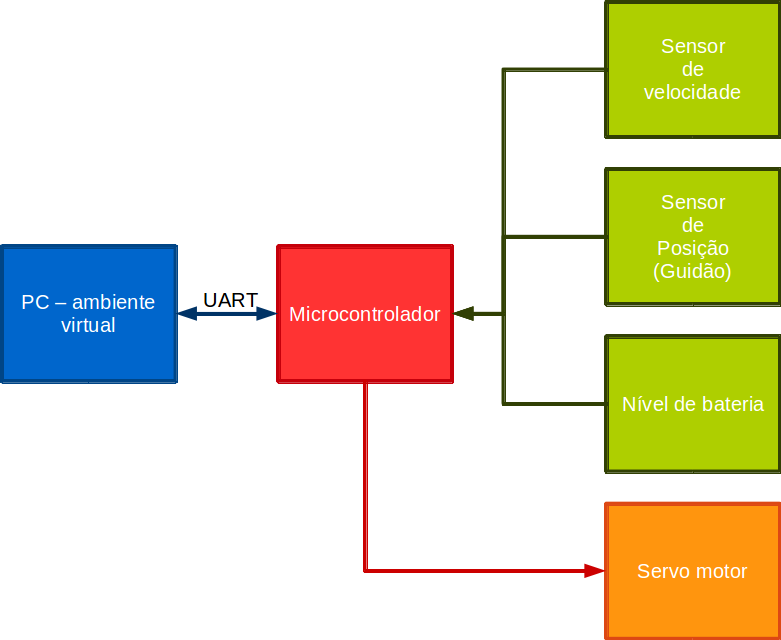
\includegraphics[width=0.8\textwidth]
      {figuras/diag_blocos_elet1.png}
  \caption{Diagrama de blocos do sistema no ponto de vista do \textit{hardware} embarcado.}
  \label{blocos}
\end{figure}

% Item sobre o projeto de software embarcado
\section{Projeto do \textit{Software} Embarcado} % (fold)
\label{sec:soft_emb}
Visando facilitar o desenvolvimento do \textit{software} a ser embarcado no microcontrolador, implementou-se uma biblioteca contendo funções para o uso especifico no \textit{kit} \textit{Launchpad}, com botões, LEDs e portas de comunicação pré definidas. Essa biblioteca contem funções básicas para entradas e saídas digitais, \textit{timer} e comunicação. Outras duas bibliotecas são utilizadas neste projeto, sendo uma para amostrar um sinal a partir do conversor A/D e outra contendo as definições do ambiente virtual.
A principio, o projeto de \textit{software} foi direcionado a leitura dos sensores do guidão, velocidade, atuador e comunicação. A seguir, serão descritas as implementações destas etapas neste projeto.

\subsection{Leitura de posição do guidão} % (fold)
\label{sub:read_guid_sens}
O sensor que verificará a posição do guidão se trata de um potenciômetro. Este dispositivo retornará um valor analógico de tensão que é proporcional a posição do guidão. Neste caso, a leitura do sinal é feita configurando-se uma entrada do microcontrolador como analógica. O valor lido tem resolução de 10 \textit{bits} e deverá estar entre 0 e 3V. A leitura deste sensor não será constante, mas sim, solicitada pelo ambiente virtual.

\subsection{Leitura de velocidade} % (fold)
\label{sub:read_vel_sens}

Para estimar a velocidade da roda traseira da bicicleta, um par transmissor-receptor de infravermelho será utilizado para calcular o período de interferência entre ambos. O sinal lido será um nível lógico (alto ou baixo)  e será obtido por uma entrada digital. Neste caso, um serviço de interrupção foi configurado para iniciar uma contagem e encerrar a mesma. O período obtido dividirá uma constante de forma a obter uma velocidade com resolução de 8 \textit{bits}. A contagem será realizada por um \textit{timer} do microcontrolador.

\subsection{Atuador no freio} % (fold)
\label{sub:read_freio_sens}

Para o controle do servomotor, implementou-se um algoritmo de PWM (\textit{pulse witdh modulation}) a partir do timer. A modulação do pulso será controlada por um valor de 1 \textit{byte} vindo do ambiente virtual. O sinal de controle gerado é transmitido por uma saída digital. O mesmo \textit{timer} será utilizado para todas as aplicações que requererem contagens. Cada contagem deverá ser de no mínimo 100us. Com o mesmo \textit{timer} foi possível emular 10 \textit{timers} via \textit{software}. Dessa forma, foi possível controlar a posição do servomotor e realizar a contagem do período do sensor de velocidade.

\section{Circuitos} % (fold)
\label{sec:circuito}

\subsection{Sensor de Posição do Guidão} % (fold)
\label{sub:poteciometro_guidao}

Para verificar o ângulo do guidão da bicicleta, o sensor que será utilizado se trata de um potenciômetro. Este dispositivo tem a capacidade de variar sua resistência em função do posicionamento de seu eixo. Este eixo será fixado no guidão da bicicleta e permitirá uma rotação de 270 graus. O potenciômetro escolhido possui uma resistência de 10k$\Omega$ e funcionará como divisor resistivo de uma tensão de 5V. O pino central fornecerá a tensão resultante deste divisor que deverá ser um valor analógico e estar entre 0 e 5V. Este sinal é condicionado por um amplificador operacional na configuração de seguidor de tensão. Por fim, a saída deste circuito é acoplada a um divisor resistivo que deverá condicionar o sinal a uma tensão entre 0 e 3V, que estão dentro da excursão de entrada do canal de entrada analógica do microcontrolador. A Figura \ref{fig:circ_pot} mostra o circuito deste sensor.

\begin{figure}[h]
  \centering
  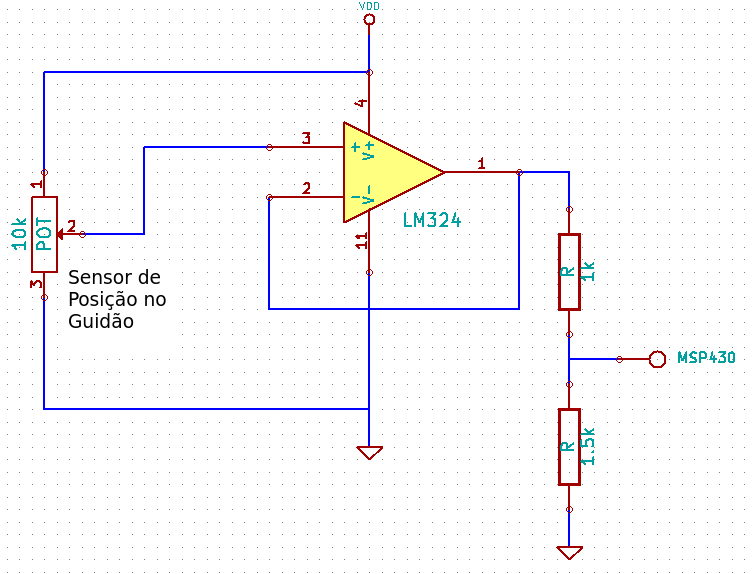
\includegraphics[width=0.8\textwidth]
      {figuras/potenciometro.png}
  \caption{Esquemático do circuito do potenciômetro.}
  \label{fig:circ_pot}
\end{figure}

\subsection{Tacômetro de Pulso} % (fold)
\label{sub:tac_metro}

O método empregado para obter a velocidade da roda foi o tacômetro de pulso. O projeto escolhido consiste em um circuito transmissor-receptor de Infravermelho, de onde será realizada uma contagem do período de não interferência entre o emissor e o receptor. Quando a interferência terminar, o microcontrolador iniciará a contagem. Esta contagem termina quando ocorre uma nova interferência. O período obtido é utilizado para obter a velocidade de transição entre os raios da roda traseira da bicicleta.

O emissor e o receptor serão instalados em suportes acoplados ao quadro da bicicleta alinhados um com o outro em lados opostos da roda. O período obtido na contagem corresponde a transição de um raio para outro, cuja distancia é de 4 cm. A Figura \ref{fig:sens_tac} mostra como será a disposição do suporte do par emissor e receptor no quadro da bicicleta. A Figura \ref{fig:figuras_tacometro} mostra o esquemático do circuito utilizado.

\begin{figure}[h]
  \centering
  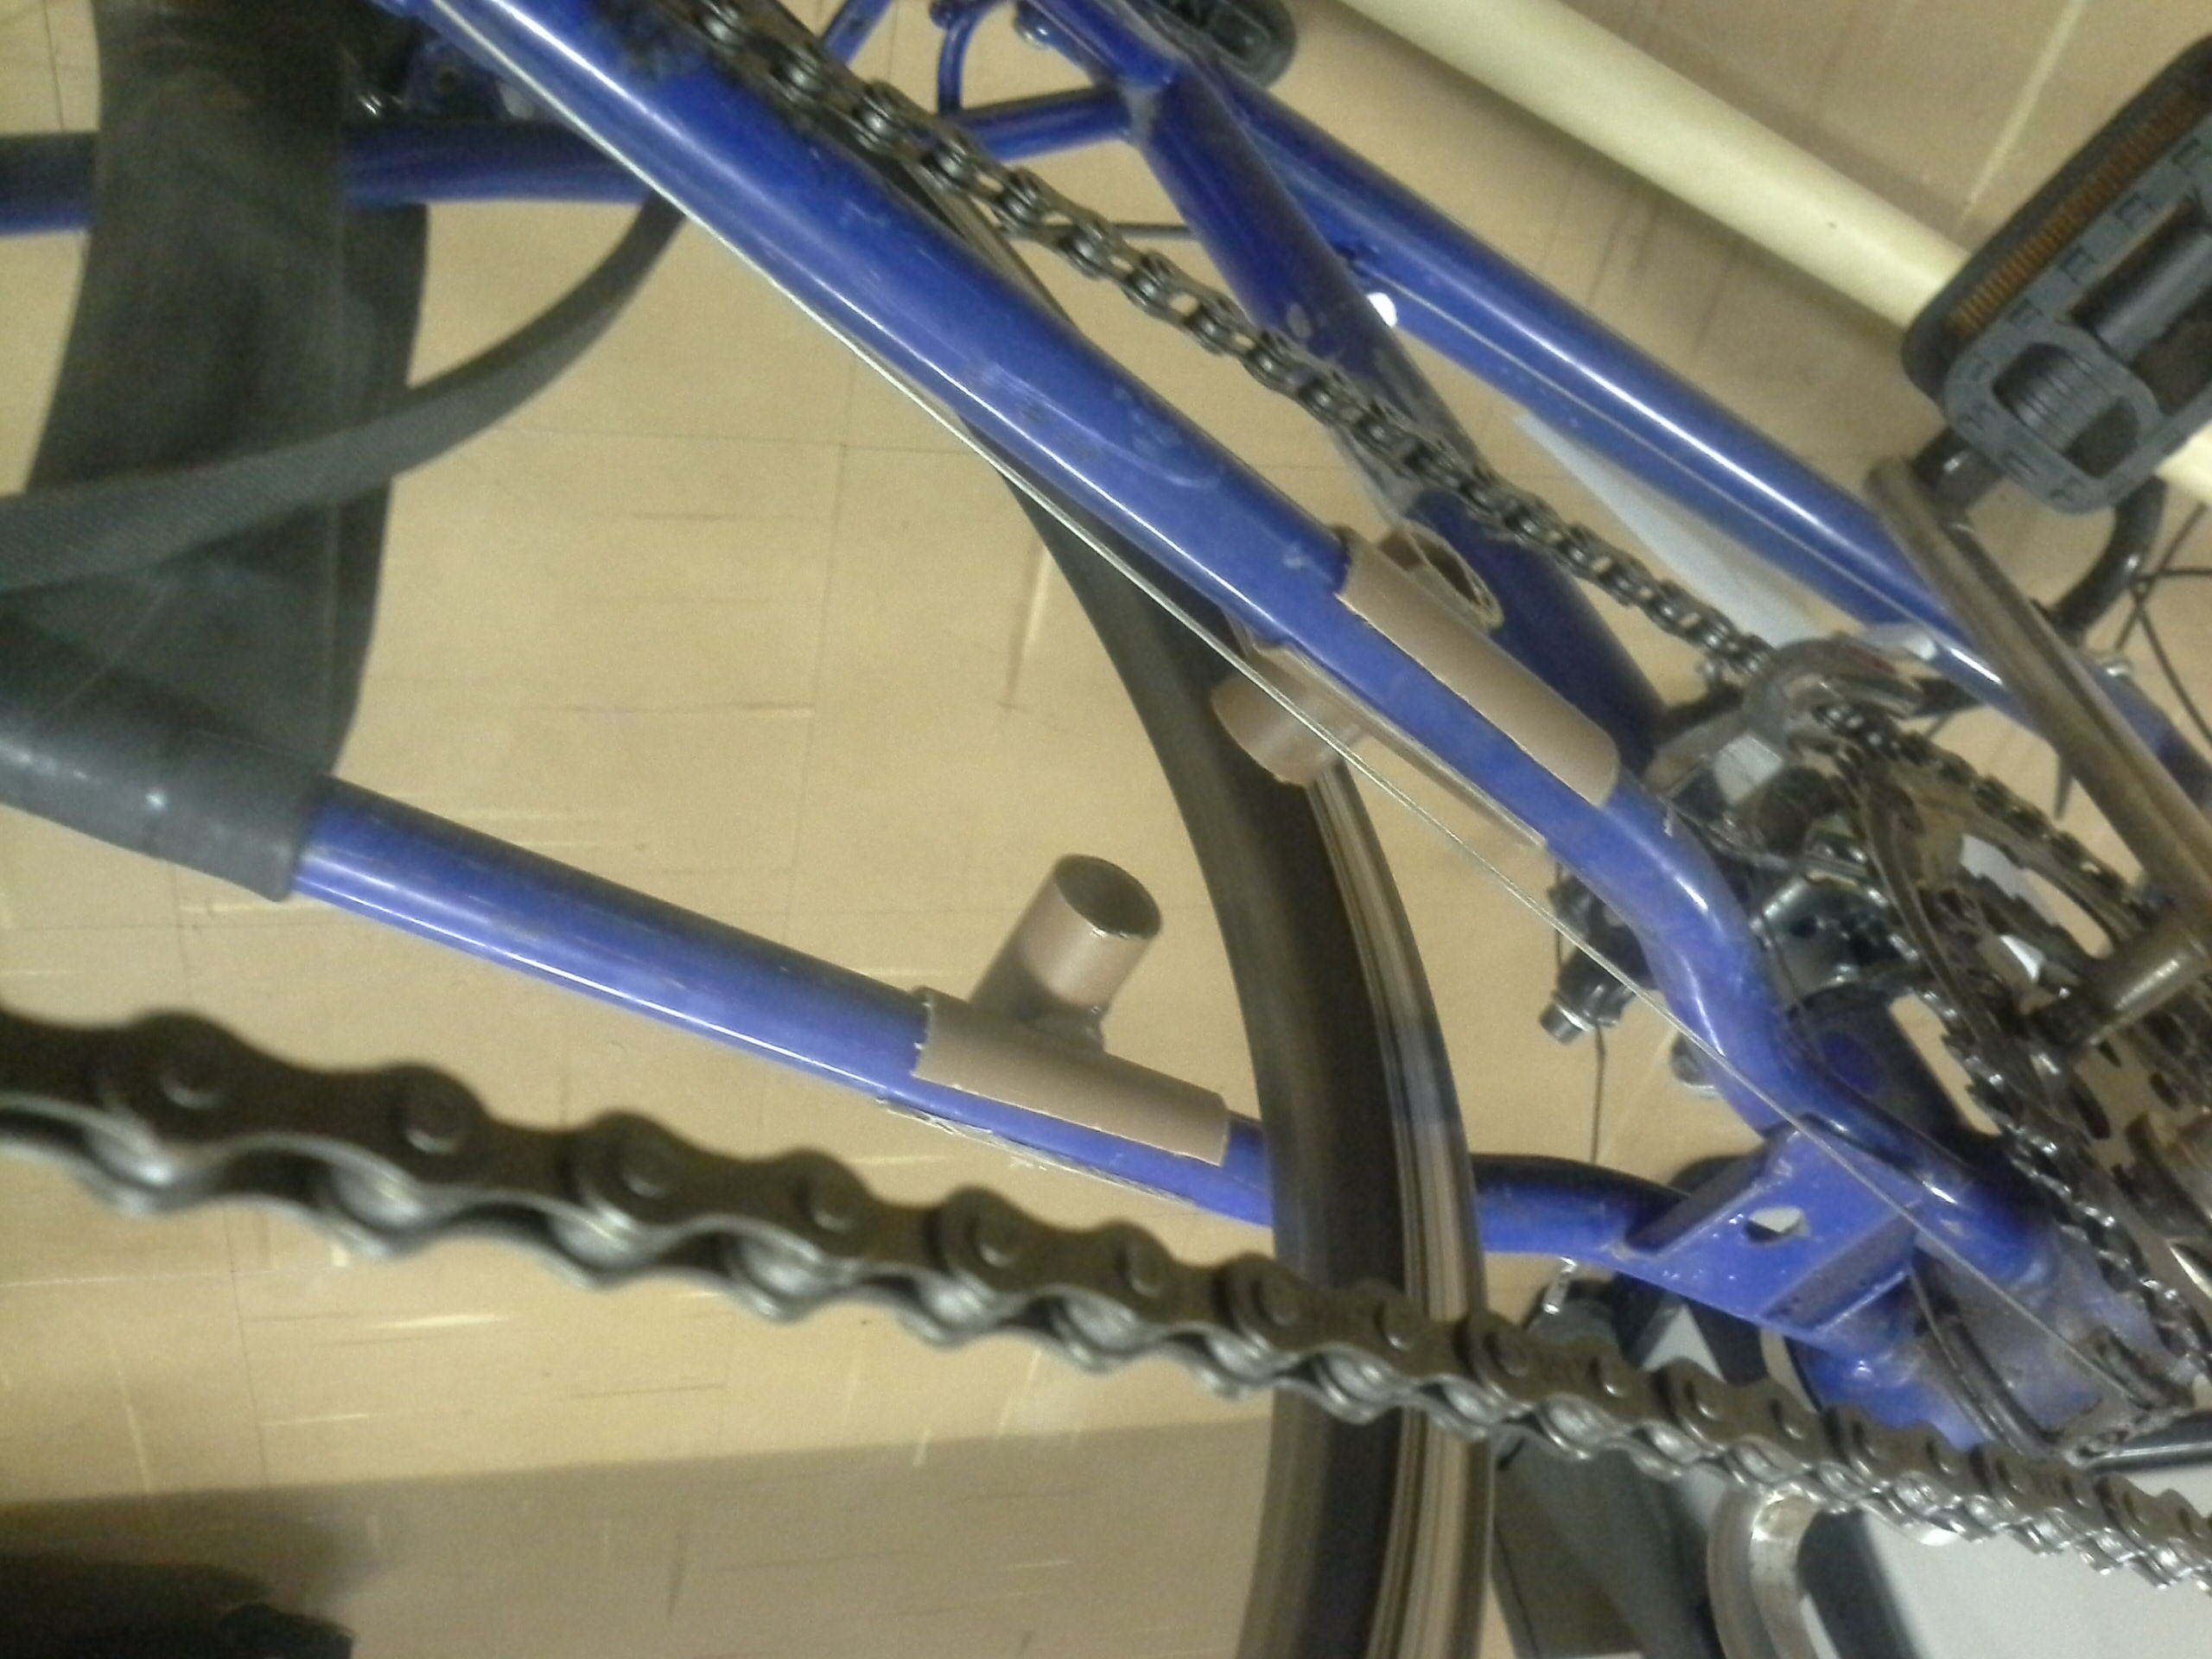
\includegraphics[width=0.8\textwidth]
      {figuras/sup_tac.jpg}
  \caption{Suporte do par transmissor-receptor de infravermelho para o tacômetro de pulso.}
  \label{fig:sens_tac}
\end{figure}

\begin{figure}[h]
  \centering
	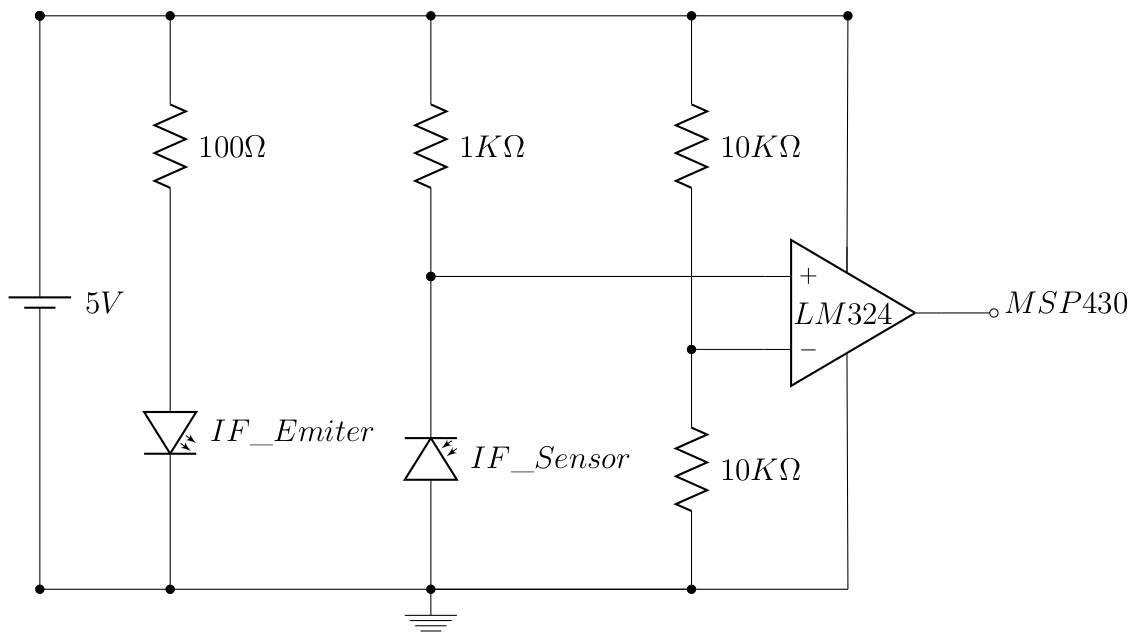
\includegraphics[width=0.8\textwidth]{figuras/tacometro}
  \caption{Circuito do Tacômetro}
  \label{fig:figuras_tacometro}
\end{figure}

% \begin{figure}[h]
% 	\centering
% 	\begin{circuitikz}[american,scale=0.7]

% 	\draw
% 	(2.5,0) node[short] (init) {}
% 	(10,-11) node[ground] (g) {}
% 	(18.1,-5.7) node[op amp,yscale=-1] (opamp){}
% 	(opamp.+) node[left] {}
% 	(17.9,-5.7) node[open]  {$LM324$}
% 	(opamp.-) node[left] {}
% 	(opamp.out) --  ++(1,0) node[ocirc,o-*] {~$MSP430$}
% 	(opamp.up) to [short] (18,-11) to (g)
% 	(opamp.down) ++ (0,.5) node[above] {} -- (opamp.down)
% 	;

% 	\draw
% 	(g) to [short] (2.5,-11) to [battery1,l_=$5V$,n=cap,*-*] ++(0,11)  to (init)
% 	(init)  to[short, *-*] (18,0) to (opamp.down)  ++(3,-3)
% 	(init)  to[short, *-*] (5,0) to [R,l^=$100\Omega$] ++(0,-5) to [empty led,l^=$IF\_Emiter$,-*] (5,-11) to (g)
% 	(init)  to[short, *-*] (10,0) to [R,l^=$1K\Omega$] ++(0,-5) to [short,n=in1,*-*] ++(0,0) 
% 	(g) to [pD,l^=$IF\_Sensor$,*-,mirror] ++(0,5) to (in1)
% 	(in1) to (opamp.+)
% 	(init)  to[short, *-*] (15,0) to [R,l^=$10K\Omega$] ++(0,-5)  to [short] ++(0,-1.40)to [short,n=in2,-*] ++(0,0) to [R,l^=$10K\Omega$,-*] (15,-11) to (g)
% 	(in2) to (opamp.-)
% 	;

% 	\end{circuitikz}
% 	\caption[Tacômetro]{Circuito do Tacômetro}
% 	\label{circ}
% \end{figure}

\subsection{Atuador do freio} % (fold)
\label{sub:atuador}

Será usado um servo motor para o controle do atuador do freio. Este servo motor é controlado por meio de uma onda PWM (\textit{Pulse Width Modulation}). Ondas PWM são usadas para controlar circuitos analógicos de forma digital, o que reduz o custo de produção e consumo do sistema. Por meio do uso de contadores de alta resolução, o \textit{duty cicle} de uma onda quadrada pode ser modulado para codificar certo valor de um sinal analógico. A tensão de controle é obtida com a constante mudança de pulsos que hora está na tensão máxima (ligado), hora está em 0 V (desligado). O tempo que este sinal fica na tensão máxima é chamado de \textit{duty cicle} de um sinal PWM (Figura \ref{fig:pwmcircuito}). Com uma repetida série de pulsos, a uma frequência satisfatória, é possível obter qualquer valor de tensão entre o máximo e mínimo valor do sinal digital.
Se um sinal PWM possui, por exemplo, 40\% de \textit{duty cicle} significa que o sinal digital está em seu valor máximo durante 40\% do seu período e está desligado durante 60\% do seu período. Caso a tensão de alimentação seja 9 V, a tensão que será medida na carga é de 40\% de 9 V, ou seja, 3,6 V.
%Atualizar figura
\begin{figure}[h]
  \centering
	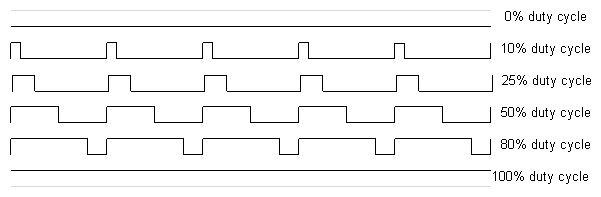
\includegraphics[width=0.8\textwidth]{figuras/pwmExample.png}
  \caption{Exemplo de sinal PWM com diferentes \textit{duty cicles}.}
  \label{fig:pwmcircuito}
\end{figure}


Como dito anteriormente, o sinal PWM deve possuir uma frequência de variação entre os pulsos de forma que a carga "veja" uma tensão analógica constante. Suponha que um sinal PWM está em seu valor máximo durante 100 ms e depois muda para 0 V e fica neste estado por outros 100 ms. Se este ciclo se repetir 60 vezes por segundo, a tensão medida na saída será de 50\% da tensão máxima com frequência de 60 Hz. A esta frequência é dado o nome de frequência de modulação e depende do tipo sistema que será controlado.
Este método foi escolhido devido a sua grande imunidade a ruído, fácil controle da tensão de saída e redução do consumo total do sistema.

O microcontrolador irá gerar o sinal PWM. Porém, seu sinal de saída precisa ser condicionado pois os níveis de tensão do microcontrolador são de 0 a 3V e o servo motor será alimentado com uma tensão de 5V. Assim, o circuito apresentado na Figura \ref{fig:circ_serv} altera os níveis lógicos de tensão para 0 a 5V. Este circuito consiste em um amplificador operacional em modo de comparação, tendo seu valor de saída sempre saturados. O servo motor será posicionado no quadro da bicicleta de forma a tracionar o cabo de aço do freio que passa pelo varão, tal como na Figura \ref{fig:foto_servo}.

\begin{figure}[h]
  \centering
	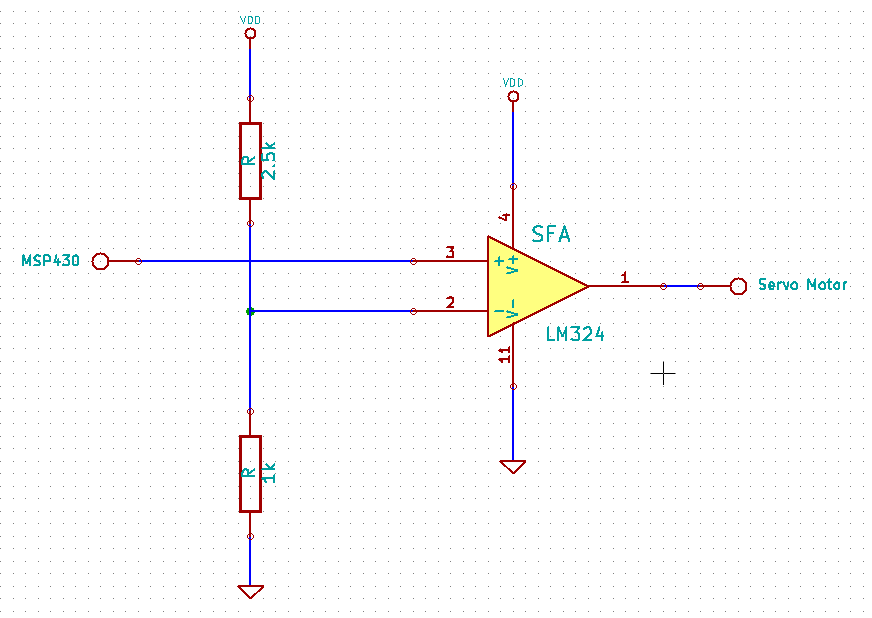
\includegraphics[width=0.8\textwidth]{figuras/circuitoPWM.png}
  \caption{Circuito utilizado para condicionar o sinal de PWM do microcontrolador para o servo motor.}
  \label{fig:circ_serv}
\end{figure}

\begin{figure}[h]
  \centering
	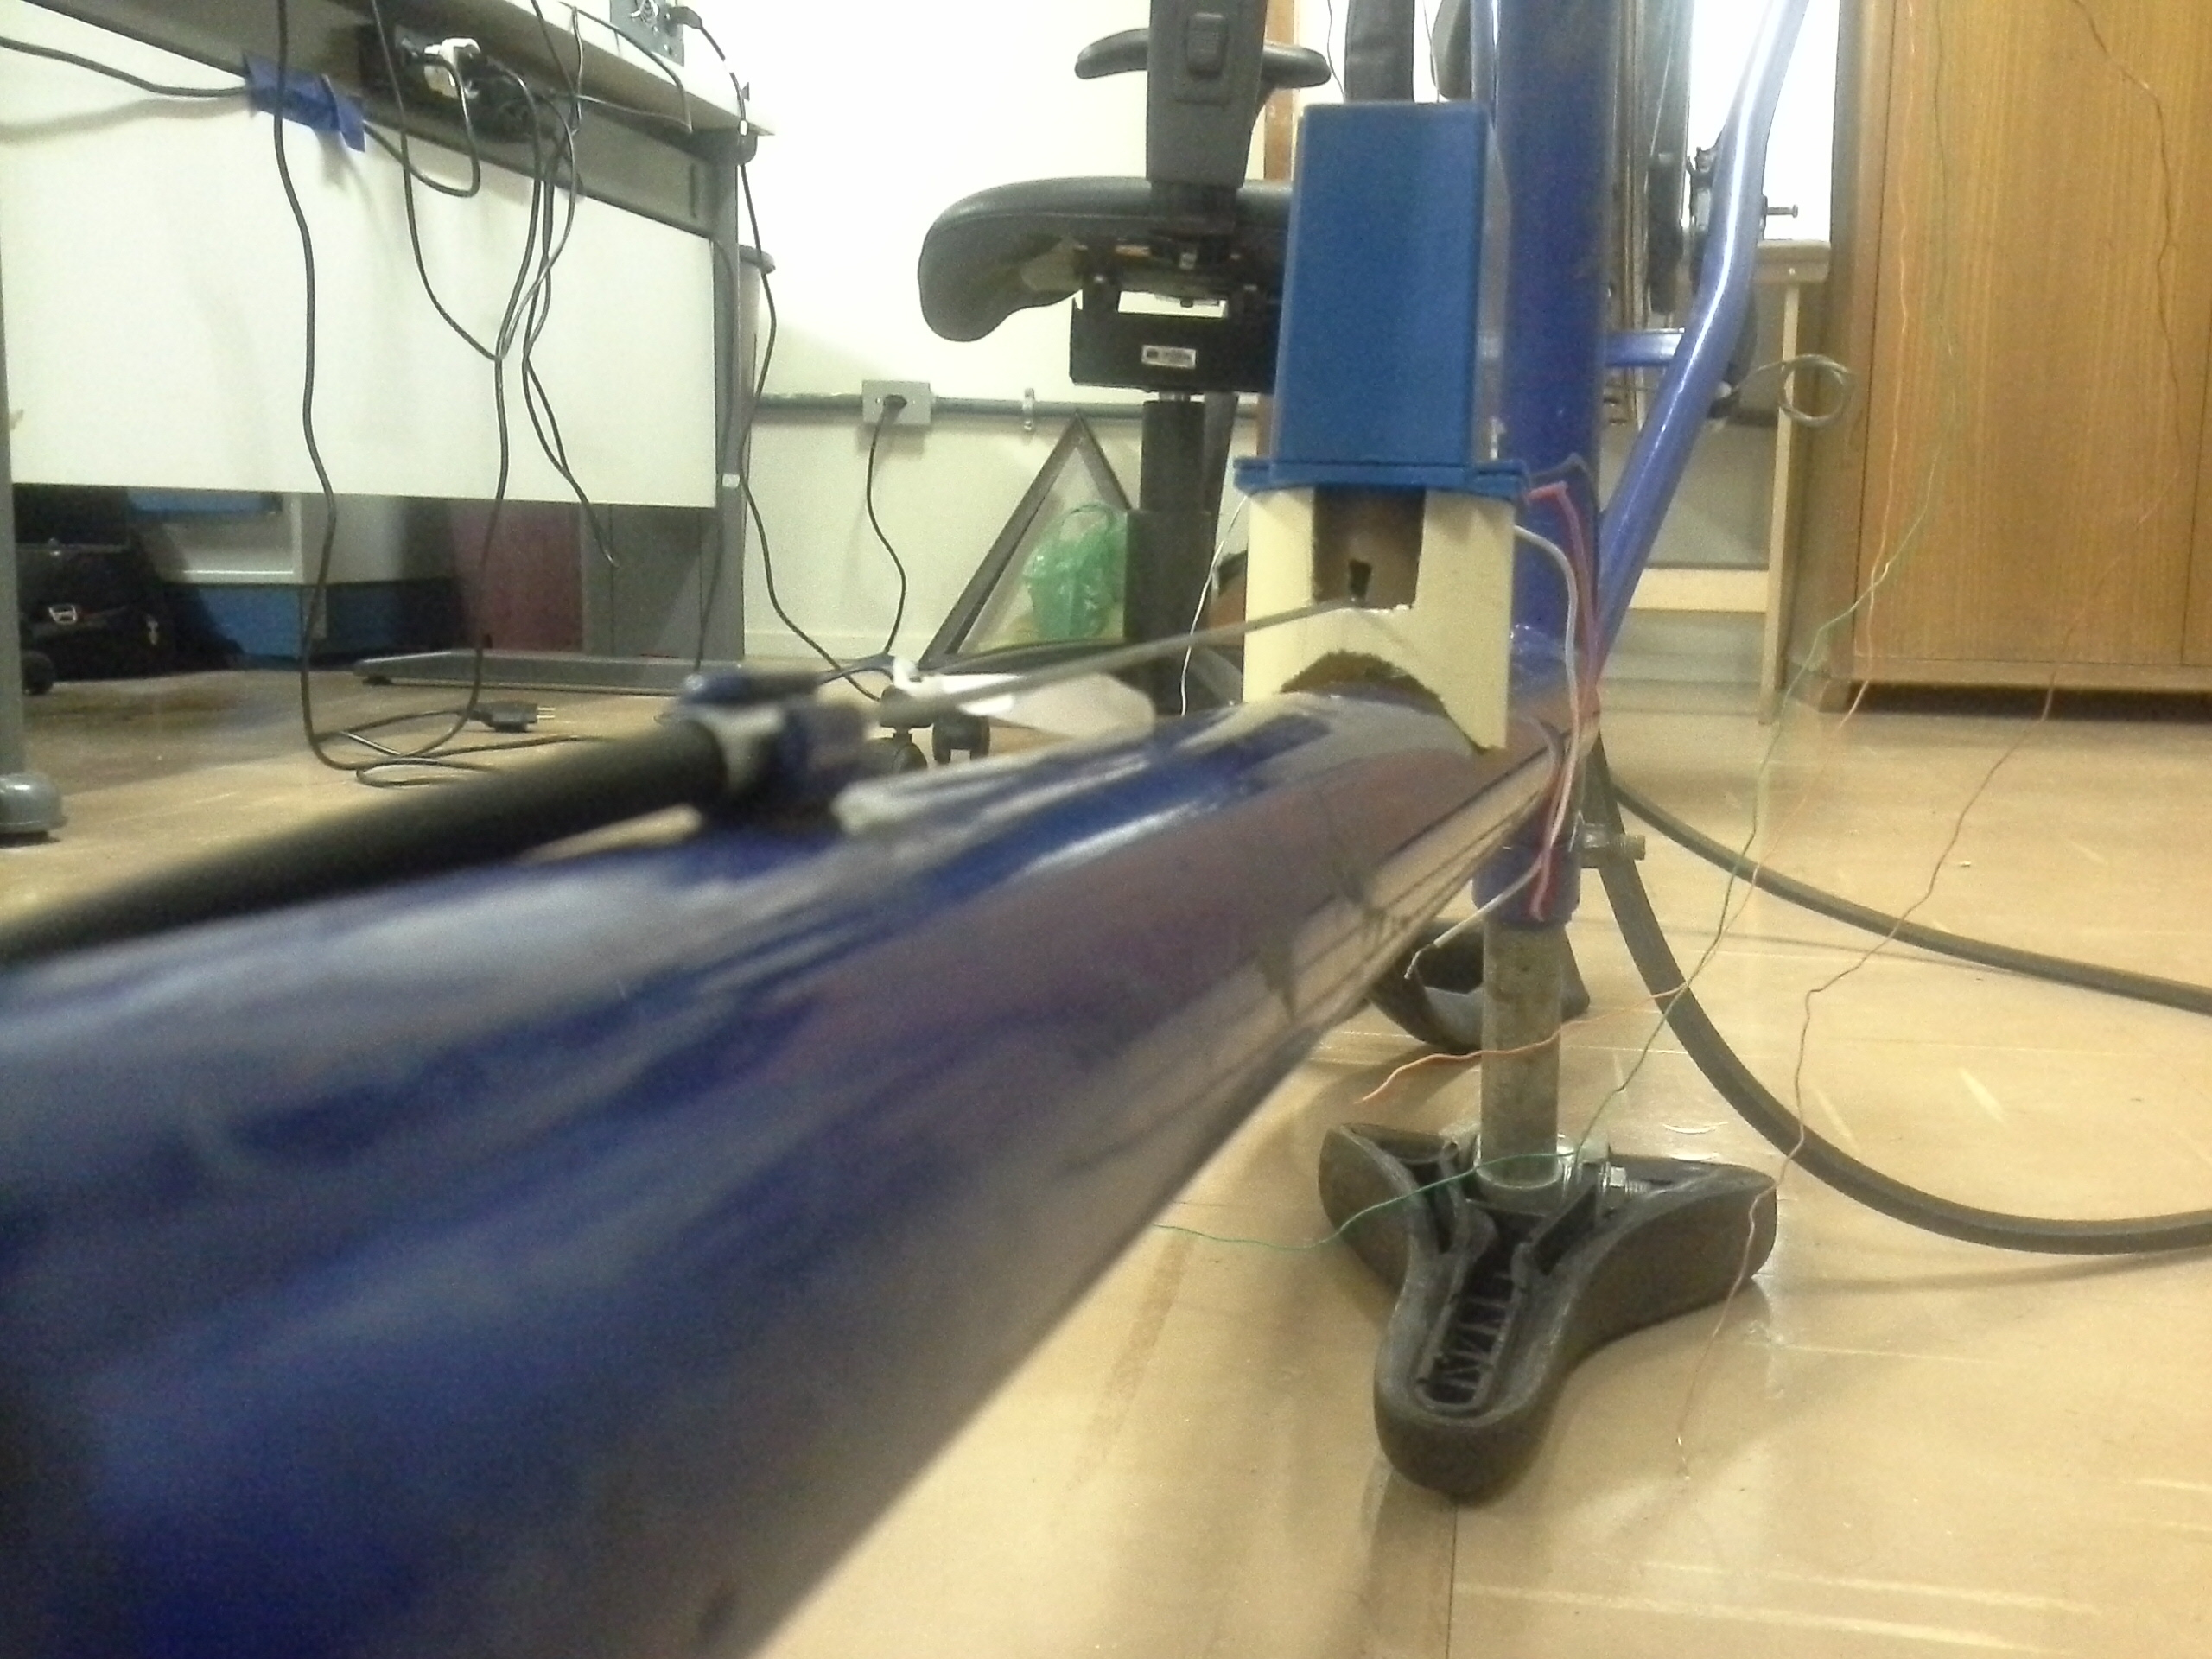
\includegraphics[width=0.8\textwidth]{figuras/servoQuadro.jpg}
  \caption{Detalhe do servo motor instalado no quadro da bicicleta.}
  \label{fig:foto_servo}
\end{figure}

\subsection{Sensor Infravermelho} % (fold)
\label{sub:sensor_infra}

Sensores Infravermelhos são detectores que possuem uma fotocélula capaz de reagir à emissão de luz infravermelha. São muito utilizado em controles remotos, teclados, mouses sem fio, bem como, no isolamento de circuitos elétricos e sensores de posição. Todos os aparelhos de TV e DVD \textit{player} possuem estes sensores para comandar alguma ação nestes aparelhos. O sinal é enviado por um LED (\textit{Light Emissor Diode}) emissor de luz infravermelha, é captado por um fototransistor e, por fim, os dados são processados. 
A aplicação destes sensores, juntos, é chamada de par ótico. Estes par ótico pode ser fabricado em diversos formatos, geralmente customizados para aplicações específicas. É possível encontrar o LED emissor e o fototransistor montados em um único encapsulamento para sensores de posição, com um sulco entre eles (Figura \ref{fig:fotoUni}), ou de forma separada funcionando como chaves óticas (Figura \ref{fig:fotoLED}), por exemplo.

\begin{figure}
        \centering
        \begin{subfigure}[b]{0.4\textwidth}
                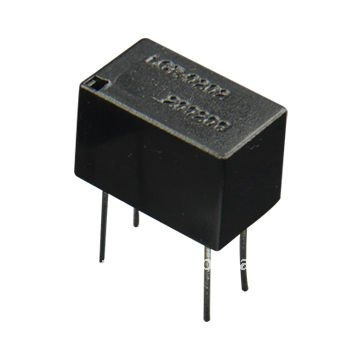
\includegraphics[width=0.7\textwidth]{figuras/optoac.jpg}
                \caption{LED e Fototransistor montados em um único encapsulamento}
                \label{fig:fotoUni}
        \end{subfigure}%
        ~
        \begin{subfigure}[b]{0.4\textwidth}
                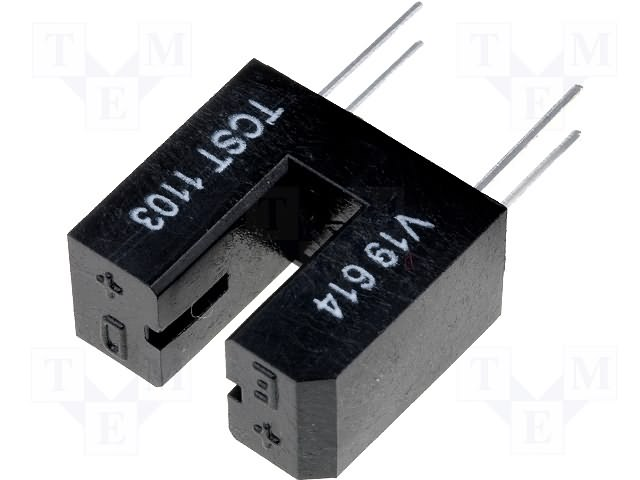
\includegraphics[width=0.7\textwidth]{figuras/opto_u.jpg}
                \caption{Fototransistor separado do LED}
                \label{fig:fotoLED}
        \end{subfigure}
        \caption{Conjuntos de LED emissor e o fototransistor}
        \label{fig:LED}
\end{figure}


%\subsection{Circuito de verificação de nível de bateria} % (fold)
%\label{sub:nivelBateria}

%Este circuito realiza a medição do nível da bateria acoplada a bicicleta que será recarregada com a energia gerada pela pedalada do usuário. O circuito se trata de um amplificador operacional configurado como circuito diferenciador. Um dos sinais de entrada é a própria fonte de alimentação do circuito, que neste caso é inicialmente de 12V. A segunda entrada recebe o sinal de um regulador de tensão de 5V, que alimentará os outros circuitos.
%Enquanto a tensão da bateria for maior que a tensão do regulador, a saída do amplificador será maior que 0. A medida em que a bateria é descarregada, sua tensão entre os polos positivo e negativo também cairá, diminuindo a diferença entre a tensão da bateria e do regulador. O status da bateria será transmitido ao usuário no ambiente virtual. A Figura \ref{fig:circ_bat} mostra o esquemático do circuito de verificação do nível da bateria.

%\begin{figure}[h]
%  \centering
%	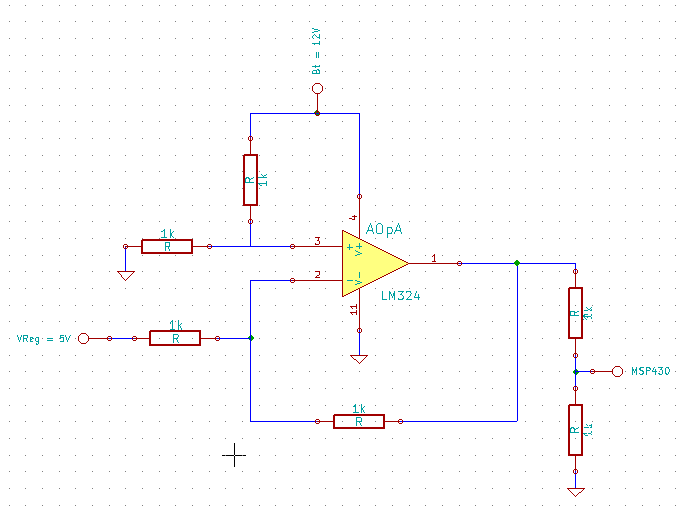
\includegraphics[width=0.8\textwidth]{figuras/circuitoBateria.png}
%  \caption{Circuito utilizado para medir o nível da bateria.}
%  \label{fig:circ_bat}
%\end{figure}



